\documentclass[UTF8,11pt]{ctexart}
\usepackage[a4paper,margin=22mm]{geometry}
\usepackage{graphicx,enumitem,amssymb,tabularx}
\usepackage[normalem]{ulem}
\usepackage{xeCJKfntef}
\setlength{\parindent}{0pt}
\setlength{\parskip}{.6em}
\sloppy
\begin{document}
\section*{2020年12月英语四级真题(第3套)}
\subsection*{\textbf{Part }I \textbf{Writing} \textbf{( 30 minutes)}}


\textbf{Directions: }\textbf{\textit{For this part, }}\textit{)OU }\textbf{\textit{are allowed 80 minutes to write on the topic Olanges in the Way of}} \textbf{\textit{Communication. You should write at least 120 words but no more than 180. words.}}


\textbf{Part ll} \textbf{Listening Comprehension} \textbf{(25 minutes)}


\noindent
\includegraphics[width=\linewidth,height=.8\textheight,keepaspectratio]{2020-12-03.assets/char-001-line-003.png}\par

\subsection*{\textbf{Part][} \textbf{Reading Comprehension} \textbf{( 40 minutes)}}


\subsection*{\textbf{Section A}}


\textbf{Directions: }\textbf{\textit{In this section, there is a passage with ten blanks. You are required to select one K/\{7;d for each}} \textbf{\textit{blank from a list of choices given in a word bank following the ptmage. Read the 'passage through carefully}} \textbf{\textit{'before making }}\textit{)OUT }\textbf{\textit{choices. E:ach choice in the bank is identified by a letter. Please mark the oorresponding}} \textbf{\textit{letter for each item on Answer Sheet 2 with a single line through the centre. You may not use any of the}}


\noindent
\includegraphics[width=\linewidth,height=.8\textheight,keepaspectratio]{2020-12-03.assets/char-001-line-007.png}\par

\textbf{The things people make, and the way they make them, determine how cities grow and decline, and}


\noindent
\includegraphics[width=\linewidth,height=.8\textheight,keepaspectratio]{2020-12-03.assets/char-001-line-009.png}\par

\textbf{disruption is surely coming. Factories are being digitised, filled} \textbf{• with new sensors and new computers to} \textbf{make them quicker, more} \textbf{\uline{27}} \textbf{, and more efficient.}


\textbf{Robots are breaking free\textperiodcentered{} from the cages that surround them, learning new skills and new ways of} \textbf{working. And 3D printers have long} \textbf{\uline{28}} \textbf{a world where you can make anything, anywhere, from a} \textbf{computerised design. That vision is} \textbf{\uline{29}} \textbf{closer to reality. These forces will lead to cleaner factories,} \textbf{producing better goods at lower prices, personalised to our individual needs and desires . -} \textbf{Humans will be}


\noindent
\includegraphics[width=\linewidth,height=.8\textheight,keepaspectratio]{2020-12-03.assets/char-001-line-012.png}\par

\textbf{life.}


\textbf{Greater efficiency} \textbf{\uline{32}} \textbf{means fewer people can do the same work. Yet faciory bosses in many}


\noindent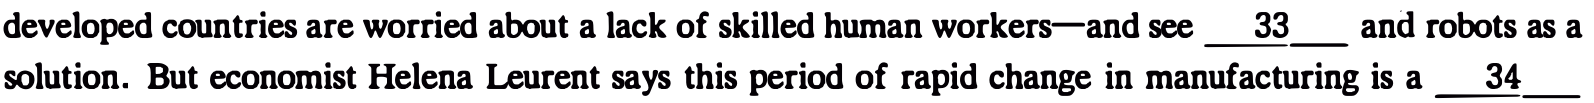
\includegraphics[width=\linewidth,height=.8\textheight,keepaspectratio]{2020-12-03.assets/char-001-line-015.png}\par

\textbf{opportunity to make the world a better place. "Manufacturing is the one system where you have got the} \textbf{biggest source of innovation, the biggest source of economic growth, and the biggest source of great jobs in} \textbf{the past. You can see it changing. That's an opportunity to} \textbf{\uline{35}} \textbf{that system differently, and if we} \textbf{can, it will hdve tremendous significance."}


\begin{itemize}[leftmargin=2em,itemsep=.2em,topsep=.4em]\item[A.] \textbf{automation}
\item[B.] \textbf{concerns}
\item[C.] \textbf{enormously}
\item[D.] \textbf{fantastic}
\item[E.] \textbf{fascinated}
\item[F.] \textbf{feature}
\item[G.] \textbf{flexible}
\item[H.] \textbf{inevitably} \textbf{\_ M) promised}
\item[I.] \textbf{interaction}
\item[J.] \textbf{leaning} \textbf{0) spared}
\item[K.] \textbf{matters}
\item[L.] \textbf{moving}
\item[N.] \textbf{shape}
\end{itemize}

\subsection*{\textbf{Section B}}


\noindent
\includegraphics[width=\linewidth,height=.8\textheight,keepaspectratio]{2020-12-03.assets/char-002-line-001.png}\par

\textbf{.} \textbf{.} \textbf{\textit{statement contains information given in one of the paragraphs }}. \textbf{\textit{Identify the paragraph from which the}} \textbf{\textit{informatio.n is derived. You may choose a paragraph more than once. Each paragraph is marked with a}} \textbf{\textit{letter; Answer the questions by marking the corresJUlding letter on Answer Sheet 2.}}


\subsection*{\textbf{The History of the Lwich Box}}


A) \textbf{It was made of shiny, bright pink plastic with a }\textbf{\textit{Little Mermaid }}\textbf{sticker oo the front, and I carried it} \textbf{with me nearly every single day. My lunch box was one of my first prized possessions, .a proud} \textbf{statement to every:one in my kindergarten: "I love Mermaid-Ariel on my lunch box."}


\textbf{\textperiodcentered{}B) That bulky container served me well through my first and second grades, until the live-action version} \textbf{of }\textbf{\textit{101 Dalmatians }}\textbf{hit theaters, and I needed the newest red plastic box with characters like Pongo and}


\subsection*{\textbf{Perdita on the front. I know I'm not alone here-I bet you loved your first lunch box, too.}}


C) \textbf{Lunch boxes have been connecting kids to cartoons and TV shows and super-heroes for decades. But it} \textbf{wasn't always that way. Once upon a time, they weren't even boxes. As schools have changed in the} \textbf{past century, the midday meal container has evolved right along with them.}


. .


\noindent
\includegraphics[width=\linewidth,height=.8\textheight,keepaspectratio]{2020-12-03.assets/char-002-line-009.png}\par

. . \textbf{While there were neighborhood schools in cities and suburbs, one-room schoolhouses were common in} \textbf{rural areas. As grandparents have been saying for generations, kids would travel miles to school in the} \textbf{countryside (often on foot).}


E) \textbf{"You had kids in rural areas who couldn't go home from school for lunch', so bringing your lunch} \textbf{wrapped in a cloth, in oiled paper, in a little wooden box or something like that was a very long-} \textbf{standing rural tradition," says Paula Johnson, \textperiodcentered{}head of food history section at the Smithsonian National} \textbf{Museum of American History in Washington, D. C.}


F) \textbf{City kids, on the other hand, went home for lunch and came back. Since they rarely carried a-meal,} \textbf{the few metal lunch buckets on the market were mainly for tradesmen and factory workers.}


G) \textbf{After World War II, a bunch of changes reshaped schoolS,--:--and lunches. More women joined the} \textbf{workforce: Small schools consolidated into larger ones, meaning more students were farther away} \textbf{from home." And the National School Lunch Act in 1946 made cafeterias much \textperiodcentered{}more common. Still,} \textbf{there wasn't much of a market for lunch containers-yet. Students who carried their lunch often did so}


\noindent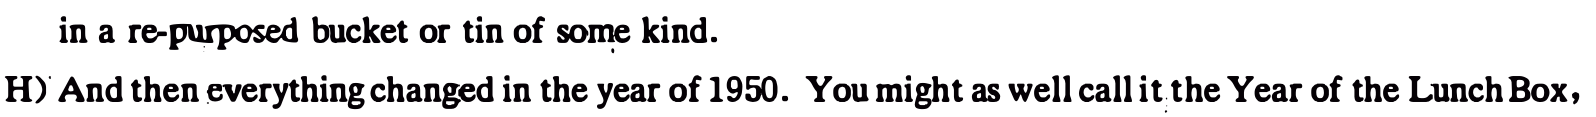
\includegraphics[width=\linewidth,height=.8\textheight,keepaspectratio]{2020-12-03.assets/char-002-line-014.png}\par

\textbf{thanks in \textperiodcentered{}large part to a genius move by a Nashville-based manufacturer, Aladdin Industries. The} \textbf{company already made square metal meal containers, the kind workers carried, and some had started} \textbf{to show up in the hands of school kids.}


I) \textbf{But these containers were really durable, lasting years on end. That was great for the consumer, not so} \textbf{much for the manufacturer. So executives at Aladdin hit on an idea that would harness the newf ound} \textbf{popularity of television. They covered lunch boxes with\textperiodcentered{} striking red paint and added a picture of TV} \textbf{and radio cowboy Hopalong Cassidy on the front.}


J) \textbf{The company sold 600,000 units the first year. It was a major" Ah-ha!" moment, and a wave of other} \textbf{manufacturers jumped on board to capitalize on new TV shows and movies. "The Partridge Family,}


\textbf{the Addams Family, the Six Million Dollar Man, the Bionic Woman-everything that was on television} \textbf{ended up on a lunch box," says Allen W,oodall. He's the founder of the Lunch Box Museum in} \textbf{Columbus, Georgia. "It was a great marketing tool because kids were taking that TV show to school}


\subsection*{\textbf{with them, and then when they got home they had them captured back on TV," he says.}}


\noindent
\includegraphics[width=\linewidth,height=.8\textheight,keepaspectratio]{2020-12-03.assets/char-003-line-002.png}\par

\textbf{Woodall has more than 2,000 items on display. His favorite? The }\textbf{\textit{Green.Hornet }}\textbf{lunch box, because he} \textbf{used to listen to the radio show back in the 1940s.}


L) \textbf{The new trend was also a great example of planned obsolescence, that is, to design a product so that it} \textbf{will soon become unfashionable or impossible to use and will need replacing. Kids would beg for a new} \textbf{lunch box every year to keep up with the newest characters, even if their old lunch box was perfectly\_} \textbf{. usable.}


M) \textbf{The metal lunch box craze lasted until the mid-1980s, when plastic took over. l\textbackslash{}vo theories exist as to} \textbf{why. The first-and most likely-is that plastic had simply become cheaper. The second theory-} \textbf{possibly an urban myth-is that concerned parents in several states proposed bans on metal lunch} \textbf{boxes, claiming kids were using them as "weapons" to hit one another. There's a lot on the internet} \textbf{about a state-wide ban in Florida, but a few days worth of digging by a historian at the Florida State} \textbf{Historical Society found no such legislation. Either way, the metal lunch box was out.}


N) \textbf{The last few decades have brought a new lunch box revolution, of sorts. Plastic boxes changed to lined} \textbf{cloth sacks, and eventually, globalism brought }\textbf{\textit{ti.ffin }}\textbf{containers from India and }\textbf{\textit{bento }}\textbf{boxes from} \textbf{Japan. Even the old metal lunch boxes have regained popularity. "I don't think the }\textbf{\textit{heyday }}\textbf{(dJ;Jle,J-JIJJ) -has passed," says D. J. Jayasekara, owner and founder of lunchbox. corn, a retailer in Pasadena,} \textbf{California. "I think it has evolved. The days of the ready-made, 'you stick it in a lunch box and carry} \textbf{it to school' are kind of done."}


\textbf{0) The introduction of backpacks changed the lunch box scene a bit, he adds. Once kids started carrying}


\noindent
\includegraphics[width=\linewidth,height=.8\textheight,keepaspectratio]{2020-12-03.assets/char-003-line-008.png}\par

\textbf{in a backpack," Jayasekara says. "It still has to go into a container." That is, in part, why smaller and} \textbf{softer containers have taken off-they fit into backpacks.} \textbf{P) And don't worry-whether it's a plastic }\textbf{\textit{bento }}\textbf{box or a cloth bag, lunch containers can still easily be} \textbf{covered with popular culture. "We keep pace with the movie industries so we can predict which} \textbf{characters are going to be popular for the coming months," Jayasekara says. "You know, kids are} \textbf{kids."}


\textbf{36. Lunch containers were not necessary for school kids in cities.}


\textbf{37. Putting TV characters on lunch boxes proved an effective marketing strategy.}


\textbf{38. Smaller lunch boxes are preferred because they fit easily. into backpacks.}


\textbf{39. Lunch boxes have evolved along with the transformation of schools.}


\textbf{40. Around the beginning of the nineteen fifties, some school kids started to use metal meal containers.}


\textbf{41. School kids are eager to get a new lunch box every year to stay in fashion.}


\textbf{42. Rural kids used to walk a long way to school in the old days.}


\textbf{43. The author was proud of using a lunch box in her childhood.}


\textbf{44. The most probable reason for the popularity of plastic lunch boxes is that they are less expensive.}


\textbf{45. The durability of metal meal containers benefited consumers.}


\subsection*{\textbf{Section C}}


\textbf{Directions: }\textbf{\textit{There are 2 passages in this section. Each passage is followed by some questions or unfinished}} \textbf{\textit{statements. For each of them there are four choices marked A), B), }}\textbf{C) }\textbf{\textit{and }}\textbf{D). }\textbf{\textit{You should decide on the}} \textbf{\textit{beJ't choice and mark the co"esponding letter on Answer Sheet 2 with a single line through the centre.}} \textbf{\textit{Pas,ageOne}}


\textbf{Questions 46 to 50 are based m the following pmage.}


\textbf{A growing number of U.S. bike riders are attracted to electric- bikes for convenience, health benefits} \textbf{and their fun factor. Although ebikes first appeared in the 90s, cheaper options and longer-lasting} \textbf{batteries are breathing new life into the concept.}


\textbf{Established bike • companies and startups are embracing ebikes to meet demand. About 34 million} \textbf{ebikes were sold worldwide last year, according to data from eCycleElectric Consultants. Most were sold} \textbf{in Europe and China, where the bikes already have exploded in popularity. Recently, the U.S. market} \textbf{has grown to 263,000 bikes, a 25\% gain from the prior year.}


\textbf{The industry is benefiting from improved batteries as suppliers over the years developed technology} \textbf{for laptops, smartphones and electric cars. In 2004, the price of batteries used on ebikes fell, spurring} \textbf{European sales.}


\textbf{But lower cost options are emerging, too. This month, three U.S. bikeshare companies, Motivate,} \textbf{LimeBike and Spin, announced electric bicycles will be added to their fleets. New York-based Jump Bikes} \textbf{is already operating an electric bikeshare in Washington, D. C., and is launching in San Francisco} \textbf{Thursday. Rides cost \$ 2 for 30 minutes.}


\textbf{The system works like existing dockless bikeshare systems, where riders unlock bikes through a} \textbf{smartphone app. "This is the beginning of a long-term shift away from regular }\textbf{\textit{pedal }}\raisebox{-0.334em}{
\includegraphics[height=1.416em]{2020-12-03.assets/char-004-001.png}}\allowbreak{}\raisebox{-0.334em}{
\includegraphics[height=1.416em]{2020-12-03.assets/char-004-002.png}}\allowbreak{}\textbf{ to electric} \textbf{bikes," said Jump Bikes CEO Ryan Rzepecki. "When people first jump on an ebike, their face lights up.} \textbf{It's exciting and joyful in a way that you don't get from a regular bike."}


\textbf{Two years ago, CEO Chris Cocalis of Pivot Cycles, which sells high-end mountain bikes, found that} \textbf{U.S. bike shops weren't interested in stocking ebikes. Some retailers warned Cocalis that they'd drop the} \textbf{brand if it came out with an electric bike.}


\textbf{Now that sales are taking off, the vast majority of bike dealers are asking Cocalis when he'll make an} \textbf{ebike available. •"There's tremendous opportunity to get a generation of people for\textperiodcentered{} whom suffering. isn't} \textbf{their thing," Cocalis said. "Ebike riders get the enjoyable part of cycling without the massive suffering of} \textbf{climbing huge hills. "}


\textbf{46. What do we learn from the passage about ebikes?}


\begin{itemize}[leftmargin=2em,itemsep=.2em,topsep=.4em]\item[A.] \textbf{Their health benefits and fun values outweigh their cost.}
\item[B.] \textbf{They did not catch public attention in the United States until the 1990s.}
\item[C.] \textbf{They did not become popular until the emergence of improved batteries.}
\item[D.] \textbf{Their widespread use is attributable to people's environmental awareness.}
\end{itemize}

\textbf{47. What brought about the boost in ebike sales in Europe at the beginning of the century?}


\begin{itemize}[leftmargin=2em,itemsep=.2em,topsep=.4em]\item[A.] \textbf{Updated technology of bike manufacture.}
\item[B.] \textbf{The falling prices of ebike batteries.}
\item[C.] \textbf{Changed fashion in short-distance travel.}
\item[D.] \textbf{The rising costs for making electric cars.}
\end{itemize}

\textbf{48. What is the prospect of the bike industry according to Ryan Rzepecki?}


\begin{itemize}[leftmargin=2em,itemsep=.2em,topsep=.4em]\item[A.] \textbf{More will be invested in bike battery research.}
\item[B.] \textbf{The sales of ebikes will increase.}
\item[C.] \textbf{It will profit from ebike sharing.}
\item[D.] \textbf{It will make a difference in people's daily lives.}
\end{itemize}

\textbf{49. What prevented Chris Cocalis from developing ebikes sooner?}


\begin{itemize}[leftmargin=2em,itemsep=.2em,topsep=.4em]\item[A.] \textbf{Retailers' refusal to deal in ebikes.}
\item[B.] \textbf{High profits from conventional bikes.}
\item[C.] \textbf{Users' concern about risks of ebike riding.}
\item[D.] \textbf{His focus on selling costly mountain bikes.}
\end{itemize}

\textbf{50. What makes Chris Cocalis believe there is a greater opportunity for ebike sales?}


\begin{itemize}[leftmargin=2em,itemsep=.2em,topsep=.4em]\item[A.] \textbf{The further lowering of ebike prices.}
\item[B.] \textbf{The public's concern for their health.}
\item[C.] \textbf{The increasing interest in mountain climbing.}
\item[D.] \textbf{The younger generation's pursuit of comfortable riding.}
\end{itemize}

\subsection*{\textbf{Passage Two}}


\textbf{Questions Sl to SS are based on the following pas.,age.}


\textbf{The terms "global warming" and "climate change" are used by many, seemingly interchangeably. But} \textbf{do they really mean the same thing?}


\textbf{Scientists shaped the history of the terms while attempting • to accurately describe how humans} \textbf{continue to alter the planet. Later, political strategists adopted the terms to influence public opinion.}


\textbf{In 1975, geochemist Wallace Broecker introduced the term "climate change"\textperiodcentered{} in an article published} \textbf{by }\textbf{\textit{Science. }}\textbf{In 1979, a National Academy of Sciences report used the term "global warming" to define} \textbf{increases in the Earth's average surface temperature, while "climate change" more broadly referred to the} \textbf{numerous effects of this increase, such as sea-level rise and ocean }\textbf{\textit{acidification }}(酸化)\textbf{.}


\textbf{During the following decades, some industrialists and politicians launched a campaign to sow doubt in} \textbf{the minds of the American public about the ability of fossil-fuel use, deforestation and other human} \textbf{activities to influence the planet's climate.}


\textbf{Word use played a critical role in developing that doubt. For example, the language and polls expert} \textbf{Frank Luntz wrote a memo encouraging the use of "climate change" because the phrase sounded less scary} \textbf{than "global warming," reported the }\textbf{\textit{Guardian.}}


\textbf{However, Luntz's recommendation wasn't necessary. A Google Ngram Viewer chart shows that by} \textbf{1993 climate change was already more commonly used in books than global warming. By the end of the} \textbf{next decade both words were used more frequently, and climate change was used nearly twice as of ten as} \textbf{global warming.}


\textbf{NASA used the term "climate change" because it more accurately reflects the wide range of changes} \textbf{to the planet caused by increasing amounts of greenhouse gases in the atmosphere.}


\textbf{The debate isn't new. A century ago, chemist Svante Arrhenius started one of the first debates over} \textbf{the potential for humans to influence the planet's climate. Arrhenius calculated the capability of carbon} \textbf{dioxide to trap heat in the Earth's atmosphere, but other chemists disagreed. Some argued that humans} \textbf{weren't producing enough greenhouse gases, while others claimed the effects would be tiny. Now, of}


\textbf{course, we know that whatever you call it, human behavior is warming the planet, with grave} \textbf{consequences ahead.}


\noindent
\includegraphics[width=\linewidth,height=.8\textheight,keepaspectratio]{2020-12-03.assets/char-006-line-001.png}\par

51. Why did politicians use the two terms "global warming'' and "climate change"?


\begin{itemize}[leftmargin=2em,itemsep=.2em,topsep=.4em]\item[A.] \textbf{To sway public opinion of the impact of human activities on Earth.}
\item[B.] \textbf{To more accurately describe the consequences of human activities.}
\item[C.] \textbf{To win more popular votes in their campaign activities.}
\item[D.] \textbf{To assure the public of the safety of existing industries.}
\end{itemize}

\textbf{52. As used in a National Academy of Sciences report, the term "climate change" differs from "global} \textbf{warming'' in that \_\_ \_}


\begin{itemize}[leftmargin=2em,itemsep=.2em,topsep=.4em]\item[A.] \textbf{it sounds less vague}
\item[B.] \textbf{it looks more scientific}
\item[C.] \textbf{it covers more phenomena}
\item[D.] \textbf{it is much closer to reality}
\end{itemize}

\textbf{53. What did industrialists of the late 20th century resort to in order to mislead Americans?}


\begin{itemize}[leftmargin=2em,itemsep=.2em,topsep=.4em]\item[A.] \textbf{Made-up survey results.}
\item[B.] \textbf{Hired climate experts.}
\item[C.] \textbf{False research findings.}
\item[D.] \textbf{Deliberate choice of words.}
\end{itemize}

\textbf{54. Why did NASA choose the term "climate change"?}


\begin{itemize}[leftmargin=2em,itemsep=.2em,topsep=.4em]\item[A.] \textbf{To obtain more funds.}
\item[B.] \textbf{For greater precision.}
\item[C.] \textbf{For political needs.}
\item[D.] \textbf{To avoid .debate.}
\end{itemize}

\textbf{55. What is the author's final conclusion?}


\begin{itemize}[leftmargin=2em,itemsep=.2em,topsep=.4em]\item[A.] \textbf{Global warming is the more accurate term.}
\item[B.] \textbf{Accuracy of terminology matters in science.}
\item[C.] \textbf{Human activities have serious effects on Earth.}
\item[D.] \textbf{Politics interferes with serious scientific debate.}
\end{itemize}

\subsection*{\textbf{Part N} \textbf{Translation} \textbf{(30 minutes )}}


\textbf{Directions: }\textbf{\textit{For this part }}, \textbf{\textit{yo.u are allowed 80 minutes to translate a passage from Chinese into English. You}} \textbf{\textit{should write yo.ur answer on .Answer Sheet 2 .}}


\noindent
\includegraphics[width=\linewidth,height=.8\textheight,keepaspectratio]{2020-12-03.assets/char-006-line-014.png}\par
\end{document}